\documentclass[12pt,letterpaper]{article}
\usepackage{graphicx} % Required for inserting images
\usepackage{listings}
\usepackage{xcolor}
\usepackage{parskip}
\usepackage{amsmath}
\usepackage{url}
\usepackage{setspace}
\onehalfspacing
\usepackage[margin=1in]{geometry}

\graphicspath{{images/}}

\title{{\vspace{-2cm}}Temporal Congestion Analysis and Predictive Modeling of Ride-Hailing Trips in NYC Using High-Volume FHV Data}
\author{Farooq Mahmud}
\date{April 25, 2025}

\definecolor{backcolor}{rgb}{0.95,0.95,0.92}

\lstdefinestyle{mystyle}{
    backgroundcolor=\color{backcolor},
    captionpos=b                  
}

\lstset{style=mystyle}

\begin{document}

\maketitle

\section{Abstract}
This study outlines a potential project to explore traffic congestion patterns in New York City by analyzing High-Volume For-Hire Vehicle (FHV) trip records from services like Uber and Lyft. Using publicly available data from all twelve months of 2024, the proposed analysis would examine how trip durations and speeds vary by time of day, day of week, and provider. After preprocessing in Apache Spark (PySpark), I plan to identify temporal trends and build predictive models in R using linear and logistic regression. The project is designed to demonstrate how the size and complexity of the dataset require the use of big data tools for processing and modeling.


\section{Introduction}
Urban traffic congestion continues to be a widespread problem that affects the efficiency of transportation systems, contributes to environmental concerns, and affects commuter well-being. In densely populated cities like New York, where ride-hailing services such as Uber and Lyft operate on a massive scale, understanding when and where congestion occurs is critical to optimizing urban mobility.

This proposed project will investigate temporal patterns in congestion using High-Volume For-Hire Vehicle (FHV) trip data collected and published by the NYC Taxi and Limousine Commission (TLC). With more than 200 million travel records from 2024 alone, the dataset provides a rich source of behavioral and operational insights. The central research question is \textit{How do trip duration and speed, as proxies of congestion, vary between different times of the day, days of the week, and ride-hailing providers?}

The objectives of this project are to (1) identify temporal congestion trends through descriptive analysis and (2) develop regression models to predict the duration of the trip or classify the trips as congested based on their characteristics. Given the volume and granularity of the dataset, traditional analysis tools fall short, necessitating the use of big data processing technologies such as Apache Spark. The goal is to produce interpretable insights that can inform urban planning, traffic policy, and ride-hailing operations.

\section{Background Review}
Riley et al. propose a scalable real-time ride-sharing architecture (A-RTRS) that integrates optimization, machine learning, and predictive model control for dynamic dispatching and vehicle relocation on idle. Their system uses time-batched optimization, historical demand forecasting, and zone-level repositioning to reduce average passenger wait times by up to 55\%. This architecture demonstrates how predictive and adaptive mechanisms can operate in large-scale, high-velocity transportation environments. \cite{riley2020dispatching}. Ma et al. present a congestion-aware optimization framework for electric ride-hailing fleets that jointly coordinates vehicle dispatching and charging operations. Their system includes a day-ahead charging plan based on time-of-use energy pricing and a reactive model that adapts to vehicle availability and charger congestion in real time. Evaluated using simulated NYC taxi data, their congestion-aware approach outperformed benchmark policies in both service rate and profit, demonstrating the impact of integrated vehicle and charging scheduling on operational efficiency. \cite{ma2024congestionaware}. These studies highlight advanced data-driven approaches to mitigating ride-hailing congestion and support the potential for predictive modeling grounded in large-scale NYC mobility data.

A growing body of research has explored the use of ride-hailing data to understand urban transportation dynamics. Previous studies have focused on topics such as demand prediction, ride-sharing optimization, pricing strategy, and transportation equity. The NYC Taxi and Limousine Commission has provided open access to large-scale trip data, which has allowed a variety of analyses, from temporal ridership patterns to spatial clustering of pick-up and drop-off zones \cite{nyctlc2023}.

Several works have used this data set to assess the impact of ride-hailing on traffic flow and use of public transit. A study by the NYU Tandon School of Engineering empirically evaluated the impact of NYC’s ride-hailing congestion surcharge policy using a difference-in-differences (DiD) approach. Although the policy led to a significant reduction in travel demand - 11\% overall, with Lyft experiencing the greatest drop - it did not result in a significant reduction in congestion. The study highlights that travel reductions were more pronounced for short-distance rides and in areas with alternative transportation options such as subways and bike sharing. It also found that the policy disproportionately affected lower income riders, raising concerns about equity and policy effectiveness\cite{nyu2023}. Although the Tandon study provides valuable insight into policy impacts using historical data, it lacks a supporting big data system architecture to enable real-time monitoring or operationalization. In contrast, the architecture proposed in this paper, which combines automated batch processing, real-time ingestion, and predictive modeling, could support dynamic congestion policy evaluation and feedback loops. Such a system could enable policy makers to monitor the impact of surcharges or routing incentives as they occur, enabling more responsive and equitable management of urban mobility. Furthermore, research from the CUNY Graduate Center examined the effects of the 2019 congestion surcharge on FHV usage in Manhattan, showing a decline in rides in charged zones \cite{cuny2023}. Although insightful, the CUNY study does not propose a scalable system for continuous or predictive policy evaluation. The big data architecture in this project would enable real-time pickup and collision monitoring, allowing faster feedback on congestion interventions and even potential automation of surcharge adjustments based on live trends. This infrastructure-oriented approach supports both exploratory and operational use cases that go beyond the economic evaluation described in the CUNY study.

Other studies have investigated the influence of surge pricing on driver behavior \cite{surgepricing2022} and analyzed pay disparities between platforms using data from 2019 to 2022 \cite{ucla2023}. However, many of these analyses are limited in scope: often examining only a few months of data, focusing exclusively on yellow taxi or green cab datasets, or lacking predictive components.

There remains a gap in the literature regarding sustained, full-year temporal analysis of congestion based specifically on High-Volume FHV data. Furthermore, predictive modeling using such data is less common, particularly models focused on estimating congestion or trip delays. This project seeks to address these shortcomings using a complete 12 month dataset and incorporating regression modeling. Furthermore, the use of big data processing tools distinguishes this study from prior work that relies on single-machine or static data approaches.

\section{Proposed Method}
This project will follow a multiphase approach consistent with the big data lifecycle, including data acquisition, preprocessing, analysis, and modeling.

\subsection{Data Acquisition and Setup}
I plan to obtain the NYC TLC High-Volume FHV trip record data set for all 12 months of 2024 \cite{dataset}. Each monthly dataset is stored in Parquet format and can be accessed via Google Drive in a cloud-based Google Colab environment. I will use Apache Spark (PySpark) for all data ingestion and transformation steps, given the dataset's scale of over 200 million records.

\subsection{Data Processing}
Data preprocessing plays a critical role in reducing both storage and compute requirements, resulting in not only time savings but also significant cost savings in a cloud-based environment. It also reduces the cognitive load on users by minimizing the number of columns they need to interpret and provides a standardized clean dataset that users can reliably use as the foundation for further analysis. By filtering out invalid records and outliers early in the pipeline, I can minimize the volume of data that needs to be processed in downstream stages, leading to more efficient use of Spark and storage resources.

In PySpark, the data will be cleaned by removing rows with null or invalid values (e.g., zero or negative durations and distances). I will create derived columns for \texttt{trip\_duration\_min}, \texttt{avg\_speed\_mph}, and categorical features like \texttt{pickup\_hour}, \texttt{pickup\_day}, and \texttt{trip\_provider}. Outliers will be filtered using interquartile range (IQR) thresholds for duration, distance, and speed of the trip. These preprocessing steps are designed to reduce noise and ensure reliable downstream analysis. 

\subsection{Operationalization and Scalability}
To transition from a one-off analysis to a production-ready system, I propose extending the workflow to support automation and real-time data ingestion. Automated preprocessing of monthly datasets can be achieved by designing a parameterized PySpark pipeline and scheduling it with tools such as Apache Airflow \cite{airflow2024}. This setup would automatically clean and transform the dataset for each new month after publication, improving efficiency and standardization. Figure \ref{fig:big-data-architecture} outlines a potential production-level architecture to support batch ingestion, scalable processing, secure storage, and model analysis.

In addition, the architecture could be extended to support real-time ingestion and streaming analytics. By integrating tools such as Apache Kafka with Spark Structured Streaming \cite{structuredstreaming2024}, the system could handle continuous data feeds from ride-hailing APIs or city sensors. This would enable use cases such as live congestion monitoring, real-time alerting, and dynamic traffic optimization. Operationalizing the pipeline in this way improves scalability and real-world applicability for continuous analytics.

\begin{figure}
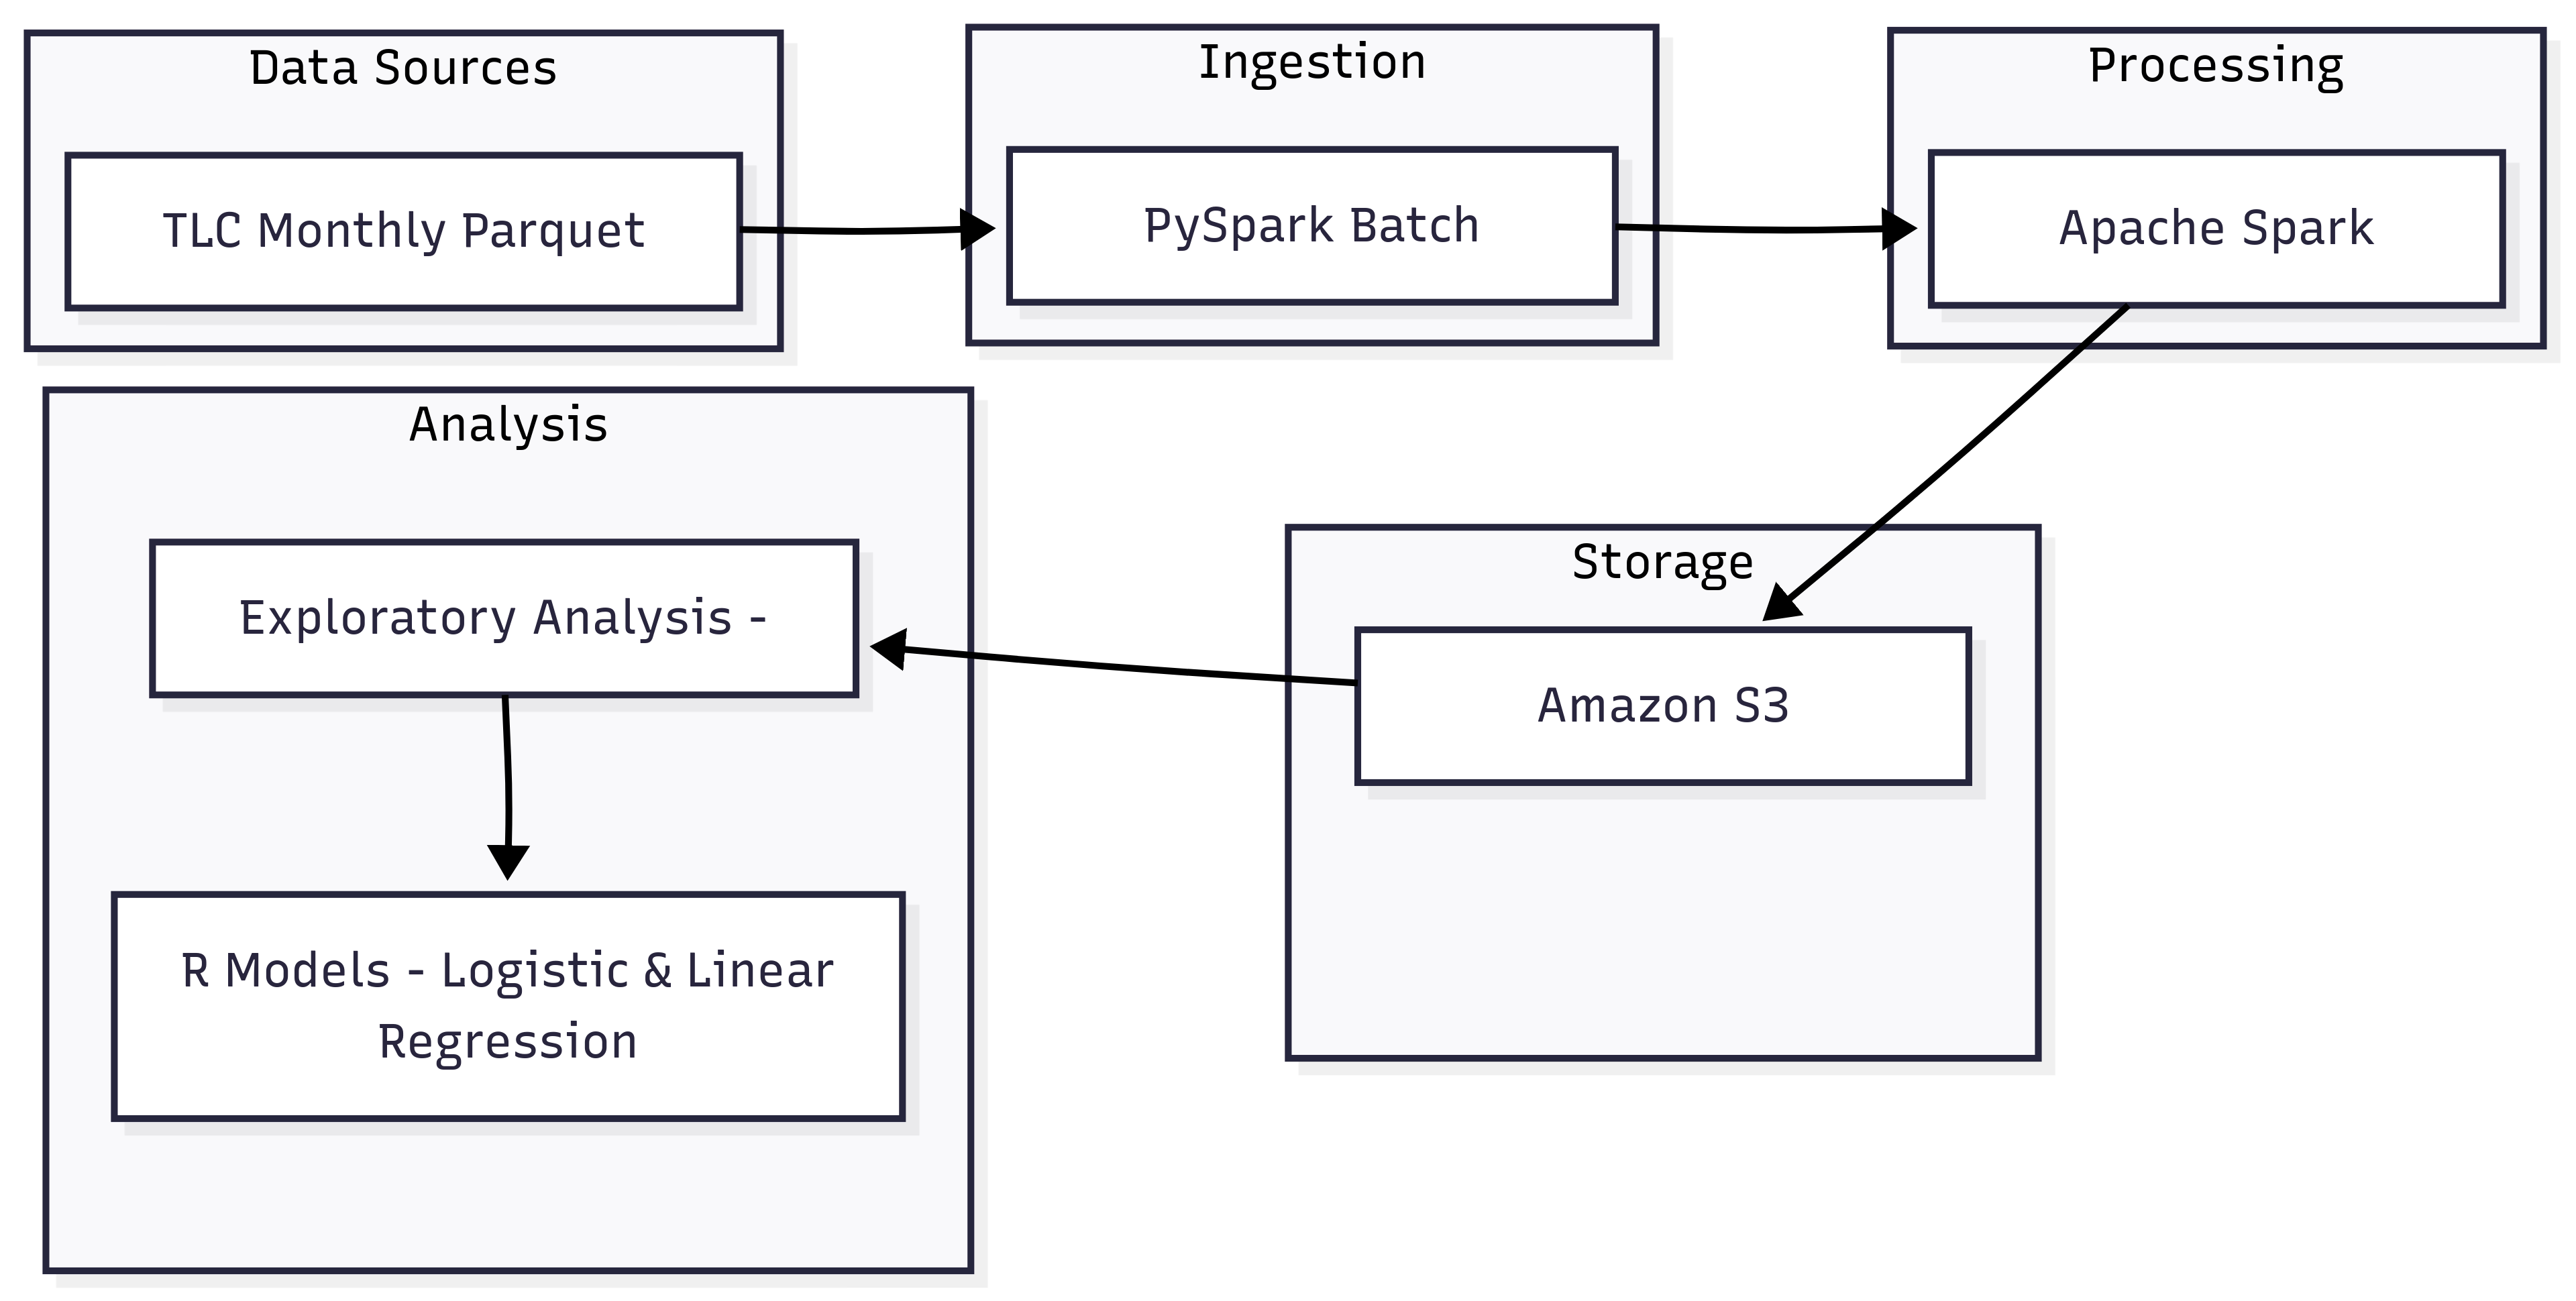
\includegraphics[width=\textwidth]{images/big-data-architecture.png}
\caption{Production-level architecture}
\label{fig:big-data-architecture}
\end{figure}


\subsection{Exploratory Analysis}
Using Spark aggregations, I plan to examine the average speed and duration of the trip by hour of day, day of week, and provider. This analysis will help identify temporal congestion patterns and inform the design of the modeling phase.

\subsection{Predictive Modeling}
The cleaned dataset can be imported into R for statistical modeling. I plan to build a multiple linear regression model to predict the duration of the trip based on characteristics such as the distance traveled, pickup hour, and the provider. In addition, I will develop a logistic regression model to classify trips as congested if their duration falls to the top 10\%. These models will be evaluated using metrics such as R-squared, accuracy, precision, and recall.

\subsection{Method Justification and Tools}
Given the volume and granularity of the dataset, traditional single-machine tools like pandas or base R would not scale. Apache Spark will enable efficient, distributed computation across the full dataset. R is proposed for its strong support for regression modeling and statistical interpretation. Together, these tools provide a scalable, interpretable, and reproducible workflow.

\subsection{Security Management}
Security is an essential consideration when designing a big data pipeline that processes public and potentially sensitive transportation data. Although the NYC TLC FHV dataset is publicly available and anonymized, future integration with private or real-time APIs may introduce data privacy and access control concerns. To ensure secure handling of data, role-based access control and data encryption should be enforced both in transit and at rest. When operationalizing the workflow in cloud environments, secure access credentials should be managed using secrets management tools such as AWS Secrets Manager \cite{awsSecretsManager2025}. In addition, audit logging and monitoring should be implemented to detect unauthorized access or anomalous usage patterns. These measures are necessary to ensure that the system adheres to data governance standards and maintains user trust.

\subsection{Storage Management}
Managing storage efficiently is critical when working with high-volume data such as NYC's FHV trip records, which can span hundreds of millions of rows annually. Choosing the right file formats, such as Parquet, for compression and efficient querying helps reduce I/O overhead and long-term storage costs. Partitioning data by month or provider can further accelerate processing in distributed computing frameworks like Apache Spark. In a production setting, storage solutions, such as Amazon S3, offer scalable and cost-effective options with integrated lifecycle policies to automate data archival or deletion \cite{awsS3}.

\section{Conclusion}
This proposed study is designed to demonstrate the value of using big data tools to analyze ride-hailing trip data to gain insight into congestion. It anticipates showing that simple predictive models can effectively estimate congestion levels using temporal features, while highlighting the importance of scalable infrastructure for large-scale mobility datasets. In future work, I may incorporate spatial features, extend modeling to multiyear data, or explore real-time streaming analysis.

\bibliographystyle{plain}
\bibliography{refs}

\end{document}
